
\chapter{Raforka og rafspenna}

Mikilvægustu stærðirnar í eðlisfræði eru svokallaðar varðveittar stærðir: orka, skriðþungi og hverfiþungi. Öflugur skilningur á þessum varðveisluhugmyndum getur oft breytt flóknu dæmi í afar einfalt dæmi! Við rifjum upp að orka er táknuð með $E$ og skilgreind þannig að:
\begin{align*}
    E = K + U
\end{align*}
Þar sem að $K = \frac{1}{2}mv^2$ táknar hreyfiorku kerfisins og $U$ táknar stöðuorku kerfisins. En stöðuorkan $U$ getur verið af margvíslegum toga og tilheyrir \emph{geymnum krafti} (sjá 5.~bekkjar námsefnið
fyrir nákvæmari skilgreiningu - en í grófum dráttum eru það allir kraftar nema núningur og loftmótsstaða). Við höfðum séð til dæmis að þyngdarkrafturinn, $F_g = -mg$, hafði tilheyrandi stöðuorku:
\begin{align*}
    U_g = mgy,
\end{align*}
þar sem að $y$ var hæð hlutarins yfir jörðu. Við höfðum einnig séð að gormkrafturinn, $F_k = -kx$, hafði tilheyrandi gormstöðuorku:
\begin{align*}
    U_k = \frac{1}{2}kx^2
\end{align*}
þar sem að $k$ var gormstuðull gormsins og $x$ var fjarlægðin frá jafnvægisstöðu gormsins (almennt er sniðugt að skilgreina stöðuorkuna þannig að hún sé núll í kraftajafnvægisstöðu kerfisins). Loks höfðum við séð að fyrir þyngdarlögmálskraftinn, $F_G = -\frac{GMm}{r^2}$, var stöðuorka þyngdarlögmálskraftsins gefin með:
\begin{align*}
    U_G = -\frac{GMm}{r}
\end{align*}
Takið eftir að stöðuorka þyngdarlögmálskraftsins er núll í $r = \infty$ og að hún er alltaf neikvæð! Hingað til höfum við alltaf haft mikið fyrir því að finna stöðuorkuna fyrir krafta. Við notuðumst þá við þá skilgreiningu að stöðuorka kraftsins væri $U = -W$ þar sem að $W$ var heildarvinnan sem að þurfti að flytja hlutinn frá jafnvægisstöðu kraftsins í punktinn sem að við ætluðum að reikna stöðuorkuna í. Það kemur í ljós að það er til einfaldari leið til þess að gera þetta með diffrun! Tökum eftir að:
\begin{align*}
    \frac{dU_g}{dy} = \frac{d}{dy}\left( mgy\right) = mg = -F_g.
\end{align*}
Eins fæst að:
\begin{align*}
    \frac{dU_k}{dx} = \frac{d}{dx}\left( \frac{1}{2}kx^2 \right) = kx = -F_k, \hspace{0.5cm} \text{og} \hspace{0.5cm} \frac{dU_G}{dr} = \frac{d}{dr}\left( -\frac{GMm}{r} \right) = -GMm \frac{d}{dr}\left( r^{-1} \right) = \frac{GMm}{r^2} = -F_G.
\end{align*}
Almennt gildir að $F = -\frac{dU}{dr}$. En ef við margföldum í gegn með $dr$ þá er $U = -\int F dr = -W$.

\newpage

\begin{tcolorbox}
\begin{theorem}
Stöðuorka rafkraftsins $F_k = \frac{kQq}{r^2}$ er gefin með:
\begin{align*}
    U_e = \frac{kQq}{r},
\end{align*}
þar sem að viðmiðunarpunktur stöðuorkunnar hefur verið skilgreindur í $r = \infty$.
\end{theorem}
\end{tcolorbox}

\textbf{Útleiðsla:} Það er einfalt mál að diffra til þess að staðfesta niðurstöðuna:
\begin{align*}
    \frac{dU_e}{dr} = \frac{d}{dr}\left( \frac{kQq}{r} \right) = kQq\frac{d}{dr}\left( r^{-1} \right) = -\frac{kQq}{r^2} = -F_k
\end{align*}
\qed

En það er óþæginlegt að burðast endalaust um með prufuhleðsluna $q$ svo að eins og fyrir rafsviðið þá skilgreinum við:

\begin{tcolorbox}
\begin{definition}
Við skilgreinum \textbf{rafspennu} stöðuorkunnar sem stærðina:
\begin{align*}
    V = \frac{U_e}{q} = \frac{kQ}{r}.
\end{align*}
\end{definition}
\end{tcolorbox}
En þar með hljóta að vera einhver tengsl við rafsviðið! Athugum að:
\begin{align*}
    F_k = -\frac{dU_e}{dr} \implies E = - \frac{dV}{dr}.
\end{align*}
Svo rafsviðið er afleiðan af rafspennunni! En fólk vill oftast frekar tala um spennumun á milli tveggja punkta. Þá er því eiginlega sama um rafspennuna sjálfa en langar bara til þess að vita hversu mikla orku þarf til þess að fara á milli tveggja punkta. En við getum fundið hvað það er með því að margfalda báðar hliðar með $dr$ og tegra frá upphafspunkintum $r = a$ í lokapunktinn, $r=b$. Við höfum þá að:
\begin{align*}
    E = -\frac{dV}{dr} \implies dV = -Edr \implies \int_{V_a}^{V_b} dV = -\int_{a}^{b} E dr
\end{align*}
Ef rafsviðið $E$ er fast þá höfum við sér í lagi að:
\begin{align*}
    \Delta V = -E(b-a).
\end{align*}
Þetta er oftast ritað þannig að heildarvegalengdin sem að hluturinn ferðast er $d = b-a$ og ef okkur er sama um formerkið á spennumuninum þá getum við skrifað:
\begin{align*}
    \Delta V = Ed
\end{align*}
Þá er sér í lagi stöðuorkubreytingin gefin með:
\begin{align*}
    \Delta U = q\Delta V = qEd.
\end{align*}
Við höfum því sýnt að:
\begin{tcolorbox}
\begin{theorem}
Í einsleitu, föstu segulsviði $E$ þá er spennumunurinn á milli tveggja punkta í fjarlægð $d$ frá hvor öðrum gefin með:
\begin{align*}
    \Delta V = Ed.
\end{align*}
Tilheyrandi stöðuorkubreyting er þá $\Delta U = q\Delta V = qEd$.
\end{theorem}
\end{tcolorbox}


\section{Plötuþéttir}


\begin{minipage}{\linewidth}
\begin{wrapfigure}{r}{1.5in}
\vspace{-0.95cm}
\includegraphics[width=1.5in]{figures/eda.pdf}
\end{wrapfigure}

Við getum beitt þessum stöðuorku- og spennumunshugmyndum á plötuþéttinn því þar höfum við einsleitt rafsvið. Rifjum upp að við höfðum til dæmis séð að í plötuþétti (sem samanstendur af tveim ferningslaga plötum með flatarmál $A$ og hleðslu $\pm Q$ í fjarlægð $d$ frá hvor annarri). Þá er rafsviðið á milli platnanna:
\begin{align*}
    E = \frac{Q}{\varepsilon_0 A}.
\end{align*}
En þar sem að það er fast þá fáum við að rafspennumunurinn á milli skauta plötuþéttisins er:
\begin{align*}
    \Delta V = Ed = \frac{Q}{\varepsilon_0 A } \cdot d = \frac{Q d}{\varepsilon_0 A}.
\end{align*}

Það er þá eðlilegt að spurja sig hvort að spennan sé meiri við jákvæða skautið eða við neikvæða skautið. Það er einföld leið til þess að svara því. Maður ímyndar sér að maður sé með jákvæðu prufuhleðsluna, $+q$. Hvert myndi hún vilja fara? Hún leitar frá jákvæðu plötunni og að neikvæðu plötunni. Þar með hefur hún meiri stöðuorku þegar hún er nær jákvæðu plötunni og minni þegar hún er nær neikvæðu plötunni. Þar með er spennan meiri nálægt jákvæðu plötunni og minni nálægt neikvæðu plötunni. Við höfum semsagt sýnt að:
\end{minipage}
\begin{tcolorbox}
\begin{theorem}
Lítum á plötuþétti með flatarmál $A$ þar sem að bilið á milli platnanna er $d$ og hleðslan á plötunum er $\pm Q$. Þá er spennumunurinn á milli platnanna gefinn með:
\begin{align*}
    \Delta V = Ed = \frac{Qd}{\varepsilon_0 A}.
\end{align*}
Spennan er meiri við jákvæðu plötuna heldur en þá neikvæðu.
\end{theorem}
\end{tcolorbox}

En það er annað sem að fólk hefur áhuga á þegar að það kemur að svona þéttum. Við skilgreinum svokallaða rýmd þéttisins sem að er mælikvarði á það hversu mikla orku þéttirinn getur geymt (við munum sjá síðar í þessum fyrirlestri hvernig það tengist orkubúskap!). Við höfum þá að:
\begin{tcolorbox}
\begin{definition}
Við skilgreinum \textbf{rýmd} þéttis með hleðslu $\pm Q$ og spennumun $V$ sem stærðina:
\begin{align*}
    C = \frac{Q}{V}.
\end{align*}
\end{definition}
\end{tcolorbox}
Þetta er reyndar oftast ritað þannig að spennumunurinn er $V = \frac{Q}{C}$. En fyrir plötuþéttinn þá þýðir þetta að:
\begin{tcolorbox}
\begin{theorem}
Rýmd plötuþéttis sem samanstendur af tveimur plötum með flatarmál $A$ sem eru í fjarlægð $d$ frá hvor anarri og bera hleðslu $\pm Q$, er gefin með:
\begin{align*}
     C = \varepsilon_0 \frac{A}{d}.
\end{align*}
\end{theorem}
\end{tcolorbox}

\textbf{Útleiðsla:} Höfðum séð að spennumunurinn var gefinn með:
\begin{align*}
    \Delta V = \frac{Qd}{\varepsilon_0 A}
\end{align*}
En þar með fáum við samkvæmt skilgreiningunni að:
\begin{align*}
    C = \frac{Q}{V} = \frac{Q}{\frac{Qd}{\varepsilon_0 A}} = \varepsilon_0 \frac{A}{d}.
\end{align*}
\qed


\section{Rafsvarar}

Hingað til höfum við (án þess að ykkur hafi verið sagt frá því) verið að vinna í tómarúmi (þar sem að rafsvörunartalan er $\varepsilon_0 = \SI{8.85e-12}{C^2/(N.m^2)}$). Hvað gerist hinsvegar þegar að við erum með rafsvið í einhverju öðru efni heldur en tómarúmi? Hvað ef við erum til dæmis með plötuþétti þar sem að er búið að leggja plastdúk inn á milli platnanna? Hvað gerist þá við rafsviðið (og rafspennuna) á milli platnanna? 

\begin{figure}[ht]
    \centering
    \includegraphics{figures/rafsvari.pdf}
\end{figure}

Það eina sem breytist er að allsstaðar þar sem að við hefðum skrifað $\varepsilon_0$ þá skrifum við $\varepsilon_{\text{efni}} \varepsilon_0$. Talan $\varepsilon_{\text{efni}}$ kallast rafsvörunartala og er háð efninu sem að rafsviðið breiðist út í gegnum. T.d.~ef við myndum setja plastdúk inn á milli tveggja platna í plötuþétti þá hefðum við $\varepsilon_{\text{plast}} = 2,3$. Í eftirfarandi töflu sjást nokkrar algengar rafsvörunartölur fyrir mismunandi efni:

\begin{table}[ht]
    \centering
    \begin{tabular}{|c|c|}
    \hline
        \textbf{Efni} & \textbf{Rafsvörunartala} \\ \hline \hline
        Tómarúm & $1$ \\ \hline
        Loft & $\SI{1.0006}{}$ \\ \hline
        Plast & $\SI{2.6}{}$ \\ \hline
        Pappír & $\SI{3.7}{}$ \\ \hline
        Olía & $\SI{4.0}{}$ \\ \hline
        Gler & $\SI{4.7}{}$ \\ \hline
        Gúmmí & $\SI{7.0}{}$ \\ \hline
        Sílíkon & $\SI{11.68}{}$ \\ \hline
        Vatn & $\SI{80.2}{}$ \\ \hline
    \end{tabular}
\end{table}
Við sjáum þá sér í lagi að $\varepsilon_{\text{efni}} \geq 1$ og þar með verður rýmd þéttisins meiri ef að við setjum rafsvara inn á milli platna plötuþéttisins. En þar sem að rafsviðið er þá gefið með:
\begin{align*}
    E_{\text{rafsvari}} = \frac{Q}{ \varepsilon_{\text{efni}} \varepsilon_0 A} \leq \frac{Q}{ \varepsilon_0 A} = E_{\text{tómarúm}}
\end{align*}
Eins fæst að spennan minnkar: $V_{\text{rafsvari}} \leq V_{\text{tómarúm}}$. Við sjáum semsagt að rafsviðið og þar með spennan ($V = Ed$ því rafsviðið er fast í plötuþéttinum) deyfast ef að við setjum einangrandi efni inn á milli platna plötuþéttisins. Hinsvegar þá stækkar rýmdin. Rýmdin er semsagt í einhverjum skilningi mælikvarði á það hversu erfitt er að búa til rafsvið á milli platnanna.




\newpage

\section{Orkuþéttleiki rafsviðsins}

Að lokum skulum við fjalla aðeins um það hversu mikil orka er í rafsviðinu. Við skulum ímynda okkur að við séum að búa til plötuþétti. Ímyndum okkur að við séum með tvær plötur sem hafa heildarhleðslu $\pm Q$ og flatarmál $A$. Hugsum okkur til að byrja með að þær séu þétt upp við hver aðra. Plöturnar finna þá fyrir aðdráttarkrafti frá hvor annarri sem er gefinn með:
\begin{align*}
    F = QE = Q \cdot \frac{Q}{2\varepsilon_0 A} = \frac{Q^2}{2 \varepsilon_0 A}
\end{align*}
Tökum eftir að þessi kraftur er fastur óháð fjarlægðinni sem að plöturnar hafa frá hvor anarri. Takið einnig eftir að tvisturinn í nefnaranum kemur til vegna þess að plöturnar finna bara fyrir rafsviðinu frá hinni plötunni, $E_{\text{plata}} = \frac{Q}{2\varepsilon_0 A}$ en ekki sínu eigin rafsviði. En þar með er vinnan sem að við þurfum að vinna til þess að færa plöturnar í sundur um vegalengd $d$ gefin með:
\begin{align*}
    W = \Vec{F} \cdot \Vec{d} = \frac{Q^2 d}{2 \varepsilon_0 A} = \frac{Q^2}{2C} = \frac{1}{2}QV  = \frac{1}{2}CV^2.
\end{align*}
Þar að auki sjáum við að $E_{\text{plötuþéttir}} = \frac{Q}{\epsilon_0 A}$ svo $Q = E A \varepsilon_0$ þannig að:
\begin{align*}
    W = \frac{1}{2} \varepsilon_0 E^2 \left(A d \right)
\end{align*}
En $Ad$ er rúmmálið sem að rafsviðið tekur. Við getum því sagt að orkuþéttleiki rafsviðsins sé gefinn með:
\begin{align*}
    u_{\!_E} = \frac{1}{2}\epsilon_0 E^2.
\end{align*}
Við álytkum semsagt að:

\begin{tcolorbox}
\begin{theorem}
Orkan, $U_C$, sem að plötuþéttir með rýmd $C$ og hleðslu $Q$ geymir er gefin með:
\begin{align*}
    U_C = \frac{Q^2}{2C}.
\end{align*}
\end{theorem}
\end{tcolorbox}


\begin{tcolorbox}
\begin{definition}
Orkuþéttleiki rafsviðsins er gefinn með:
\begin{align*}
    u_{\!_E} = \frac{1}{2}\varepsilon_0 E^2.
\end{align*}
\end{definition}
\end{tcolorbox}
Athugum þá sér í lagi að eining er: $\left[ u_{\!_E} \right] = \frac{\si{J}}{\si{m^3}}$.

\section{Klassískur geisli rafeindarinnar (*)}

En þá höfum við einfalda leið til þess að finna geisla róteindarinnar. Látum róteindina hafa geisla $r_p$. Þá höfum við að heildarorka hennar, $U$, vegna rafsviðsins er gefin með:
\begin{align*}
    U = \frac{1}{2}\epsilon_0 E^2 \cdot \frac{4\pi}{3} r_p^3
\end{align*}
En samkvæmt lögmáli Gauss getum við fundið rafsviðið með:
\begin{align*}
    \oint \Vec{E} \cdot d\Vec{A} = \frac{e}{\epsilon_0} \implies E = \frac{e}{\epsilon_0 4\pi r_p^2}
\end{align*}
sem gefur okkur því að:
\begin{align*}
    U = \frac{1}{2} \epsilon_0 \cdot \frac{e^2}{\epsilon_0^2 16\pi^2 r_p^4} \cdot \frac{4\pi}{3} r_p^3 \implies r_p = \frac{ke^2}{6 U}
\end{align*}
En samkvæmt Einstein er $U = m_p c^2$ svo við fáum:
\begin{align*}
    r_p = \frac{ke^2}{6m_p c^2} \approx \SI{2.6e-19}{m}
\end{align*}
Eins getum við sýnt að geisli rafeindar er gefinn með:
\begin{align*}
    r_e = \frac{ke^2}{6 m_e c^2} \approx \SI{0.47e-15}{m}
\end{align*}

\newpage

\section{Dæmi}


\subsection*{Dæmatími 8: Rafstöðuorka}

\begin{tcolorbox}
Rafstöðuorkan er $U = qV$ þar sem $q$ er hleðslan og $V$ er rafspennan.
\end{tcolorbox}

\begin{enumerate}[label = \textbf{(\alph*)}]

\item[\textbf{(25.12)}] Hver er hraði rafeindar sem hefur verið hraðað yfir $\Delta V = \SI{1000}{V}$ spennumun?

\item[\textbf{(25.13)}] Hversu mikinn spennumun, $\Delta V$, þarf til þess að hraða rafeind úr $v_0 = \SI{0}{m/s}$ í $v = \SI{2.0e6}{m/s}$?

\item[\textbf{(25.16)}] Rafeind með upphafshraða $v_0 = \SI{5.0e5}{m/s}$ stöðvast við það að ferðast í gegnum einsleitt rafsvið í plötuþétti.
\begin{enumerate}[label = \textbf{(\alph*})]
    \item Ferðaðist rafeindin í áttina að hærri eða lægri spennu?
    \item Hver er spennumunurinn á milli upphafsstaðsetningu rafeindarinnar og lokastaðsetningu hennar?
\end{enumerate}

\item[\textbf{(25.20)}] Eðlisfræðingar nota oft eininguna $\si{eV}$ (electron-volt) þegar þeir glíma við orku kjarneinda. Einingin er skilgreind þannig að $\SI{1}{eV}$ jafngildir orkunni sem þarf til þess að hraða rafeind yfir spennumun $\Delta V = \SI{1}{V}$.
\begin{enumerate}[label = \textbf{(\alph*)}]
    \item Hvað samsvarar $\SI{1}{eV}$ mörgum Joulum?
    \item Hver er hraði róteindar sem hefur hreyfiorku $K = \SI{5000}{eV}$?
\end{enumerate}

\end{enumerate}

\begin{tcolorbox}
\begin{enumerate*}[label = \vspace{0.15cm} ]
  \item \textbf{(25.12)} $v = \SI{1.9e7}{m/s}$.
  \item \textbf{(25.13)} $V = \SI{11.4}{V}$.
  \item \textbf{(25.16)} $\Delta V = \SI{-0.71}{V}$.
  \item \textbf{(25.20)} $\SI{1}{eV} = \SI{1.602e-19}{J}$, $v = \SI{4.2e7}{m/s}$.
\end{enumerate*}
\end{tcolorbox}

\newpage

\subsection*{Dæmatími 9: Rafspenna}

\begin{tcolorbox}
Rafspenna punkthleðslu, $Q$, er gefin með: $V = \frac{U}{q} = \frac{kQ}{r}$. Til samanburðar er rafsvið punkthleðslu gefið með $\vec{E} = \frac{\vec{F}}{q} = \frac{kQ}{r^2}\hat{r}$.
\end{tcolorbox}

\begin{enumerate}[label = \textbf{(\alph*)}]

\item[\textbf{(25.30)}] Hver er rafspennan í svarta punktinum á myndinni hér fyrir neðan?

\begin{figure}[H]
    \centering
    \includegraphics{figures/rk2530.pdf}
\end{figure}

\item[\textbf{(25.31)}] Hver er rafspennan í svarta punktinum á myndinni hér fyrir neðan?

\begin{figure}[H]
    \centering
    \includegraphics{figures/rk2531.pdf}
\end{figure}

\item[\textbf{(25.32)}] Rafspennan í svarta punktinum á myndinni hér fyrir neðan er $\SI{3140}{V}$. Hvert er gildið á hleðslunni, $q$?

\begin{figure}[H]
    \centering
    \includegraphics{figures/rk2532.pdf}
\end{figure}

\item[\textbf{(25.33)}] Tvær hleðslur, $\pm q = \pm \SI{2.0}{nC}$ eru staddar í $x = \pm \SI{1.0}{cm}$. 
\begin{enumerate}[label = \textbf{(\alph*)}]
    \item Hvar (ef einhversstaðar) á $x$-ásnum er rafsviðið núll?
    \item Hvar (ef einhversstaðar) á $x$-ásnum er rafspennan núll?
    \item Teiknið graf sem sýnir $E$ sem fall af $x$ og graf sem sýnir $V$ sem fall af $x$.
\end{enumerate}

\end{enumerate}

\begin{tcolorbox}
\begin{enumerate*}[label = \vspace{0.15cm} ]
  \item \textbf{(25.30)} $V_D = \SI{870}{V}$.
  \item \textbf{(25.31)} $V_D = \SI{-1560}{V}$.
  \item \textbf{(25.32)} $q = \SI{10}{nC}$.
  \item \textbf{(25.33)} Sjá gröf í lausnum.
\end{enumerate*}
\end{tcolorbox}

\newpage

\subsection*{Dæmatími 10: Þéttar}

\begin{tcolorbox}
Rafsviðið í þétti er gefið með: $E = \frac{Q}{\varepsilon_0 A}$. Þar sem að rafsviðið er einsleitt þá verður rafspennan: $V = Ed = \frac{Qd}{\varepsilon_0 A}$ í plötuþéttinum. Við skilgreinum þá yfirleitt rafspennuna þannig að hún sé núll við neikvæðu plötuna og $V = qEx$ þar sem $x$ er fjarlægðin frá neikvæðu plötunni. Spennumunurinn yfir plötuþéttinn er þá $\Delta V = qEd$ þar sem $d$ er plötubilið.
\end{tcolorbox}

\begin{enumerate}[label = \textbf{(\alph*)}]

\item[\textbf{(25.22)}] \begin{enumerate}[label = \textbf{(\alph*)}]
    \item Hver er spennan á AA og AAA rafhlöðum?
    \item Tengjum AA rafhlöðu við plötuþéttir sem hefur hliðarlengdir $\ell = \SI{4.0}{cm}$ og plötubil $d = \SI{1.0}{mm}$. Hversu mikla hleðslu fær þá hvor plata um sig frá rafhlöðunni?
\end{enumerate}

\item[\textbf{(25.23)}] Plötuþéttir með geisla $r = \SI{1.5}{cm}$ hefur plötubil $d = \SI{2.0}{mm}$. Rafsviðið í þéttinum er $E = \SI{1.0e5}{V/m}$. 
\begin{enumerate}[label = \textbf{(\alph*)}]
    \item Hver er spennumunurinn á milli platnanna?
    \item Hver er hleðslan á plötunum?
\end{enumerate}

\item[\textbf{(25.25)}] Tvær plötur með geisla $r = \SI{1.0}{cm}$ eru í fjarlægð $d = \SI{2.0}{mm}$ frá hvor annarri. Rafsviðið á milli þeirra er $E = \SI{5.0e5}{V/m}$.
\begin{enumerate}[label = \textbf{(\alph*)}]
    \item Hver er spennan yfir þéttinn?
    \item Rafeind er skotið frá neikvæðri plötunni með upphafshraða $v_0$. Hún lendir á jákvæðu plötunni með hraða $v = \SI{2.0e7}{m/s}$. Hver var upphafshraði rafeindarinnar? 
\end{enumerate}

\item[\textbf{(25.26)}] Róteind er skotið frá miðjunni á plötuþétti í áttina að jákvæðu plötunni með upphafshraða $v_0 = \SI{2.0e5}{m/s}$. Spennumunurinn á milli platnanna er $\Delta V = \SI{500}{V}$.

\begin{enumerate}[label = \textbf{(\alph*)}]
    \item Sýnið að upphafshraði róteindarinnar er ekki nægilegur til þess að róteindin nái að snerta jákvæðu plötuna.
    \item Hver verður hraði róteindarinnar þegar hún snertir jákvæðu plötuna?
\end{enumerate}

\end{enumerate}

\begin{tcolorbox}
\begin{enumerate*}[label = \vspace{0.15cm} ]
  \item \textbf{(25.22)} $V = \SI{1.5}{V}$, $Q = \SI{21}{\mu C}$.
  \item \textbf{(25.23)} $V = \SI{200}{V}$, $Q = \SI{0.63}{nC}$.
  \item \textbf{(25.25)} $\Delta V = \SI{1000}{V}$, $v_0 = \SI{6.95e6}{m/s}$.
  \item \textbf{(25.26)} $v_1 = \SI{2.97e5}{m/s}$.
\end{enumerate*}
\end{tcolorbox}

\newpage

\subsection*{Dæmatími 11: Rýmd þéttis og rafsvarar}


\begin{tcolorbox}
Rýmd er skilgreind sem stærðin $C = \frac{Q}{V}$. Fyrir plötuþétti þýðir þetta að í tómarúmi gildir að: $C_{\text{plötuþéttir}} = \varepsilon_0 \frac{A}{d}$. Hinsvegar ef að við setjum eitthvað efni inn á milli platnanna þá deyfist rafsviðið. Við segjum þá að efnið hafi einhvern rafsvörunarstuðul, $\varepsilon_{\text{efni}}$ og rýmd plötuþéttis með rafsvara er þá gefin með: $C_{\text{plötuþéttir}} = \varepsilon_{\text{efni}} \varepsilon_0 \frac{A}{d}$.
\end{tcolorbox}

\begin{enumerate}[label = \textbf{(\alph*)}]

\item[\textbf{(26.21)}] Tvær hringlaga álplötur með geisla $r = \SI{2.5}{cm}$ eru í fjarlægð $d = \SI{1}{mm}$ frá hvor annarri. Rafhlaða sem er tengd við báðar hliðar þéttisins býr til spennumun $\Delta V = \SI{90}{V}$ á milli platnanna.

\begin{enumerate}[label = \textbf{(\alph*)}]
    \item Hver er rýmd þéttisins?
    \item Hver er hleðslan á plötunum?
\end{enumerate}

\item[\textbf{(26.23)}] Við ætlum að smíða plötuþétti með rýmd $C = \SI{100}{pF}$. Við ætlum að nota plötur með hliðarlengdir $\ell$ og ætlum að setja litlar plastþynnur í hornin á plötunum til þess að búa til plötubilið. Plastþynnurnar hafa þykkt $þ = \SI{0.20}{mm}$. Hvernig eigum við að velja $\ell$?

\item[\textbf{(26.35)}] Tvær plötur með hliðarlengdir $\ell = \SI{4.0}{cm}$ hafa verið aðskildar með plötubili $d = \SI{0.20}{mm}$ með því að setja Teflon-dúk inn á milli platnanna. Rafsvörunarstuðull teflons er $\varepsilon_{\text{teflon}} = \SI{2.1}{}$ og mesta rafsviðið sem er hægt að ná inni í tefloni er $E_{\text{max,teflon}} = \SI{6.0e6}{V/m}$.
\begin{enumerate}[label = \textbf{(\alph*)}]
    \item Hver er rýmd þéttisins?
    \item Hver er mesti hugsanlegi spennumunurinn á milli platnanna?
\end{enumerate}

\item[\textbf{(26.36)}] Tvær plötur með hliðarlengdir $\ell = \SI{5.0}{mm}$ hafa verið aðskildar með plötubili $d = \SI{0.10}{mm}$ frá hvor annarri. Plötuþéttirinn er tengdur við $\SI{9.0}{V}$ rafhlöðu. Síðan er $\SI{0.10}{mm}$ þykku lagi af Mylar ($\varepsilon_{\text{Mylar}} = \SI{3.1}{}$) komið fyrir á milli platnanna (án þess að aftengja rafhlöðuna). Hver verður spennumunurinn, rafsviðið og hleðslan á þéttinum \textbf{(a)} áður en Mylar-lagið er sett inn á milli platnanna \textbf{(b)} eftir að Mylar lagið er sett inn á milli platnanna.
\end{enumerate}


\begin{tcolorbox}
\begin{enumerate*}[label = \vspace{0.15cm} ]
  \item \textbf{(26.21)} $C = \SI{17.4}{pF}$, $Q = \SI{1.57}{nC}$.
  \item \textbf{(26.23)} $\ell = \SI{4.75}{cm}$.
  \item \textbf{(26.35)} $C = \SI{149}{pF}$, $V = \SI{12000}{V}$.
  \item \textbf{(26.36)} $V_0 = \SI{9.0}{V}$, $Q_0 = \SI{19.8}{pC}$, $E_0 = \SI{90}{kN/C}$, $V_{\!_M} = \SI{9.0}{V}$, $Q_{\!_M} = \SI{61.2}{pC}$, $E_{\!_M} = \SI{29}{kN/C}$. 
\end{enumerate*}
\end{tcolorbox}

\newpage

\subsection*{Dæmatími 12: Orkan í þétti}

\begin{tcolorbox}
Krafturinn sem að önnur plata plötuþéttisins togar í hina með er gefinn með $F = QE = Q \cdot \frac{Q}{2 \varepsilon_0 A}$. En þá er vinnan sem að þarf til þess að búa til plötuþétti gefin með:
\begin{align*}
    W = \vec{F} \cdot \vec{d} = \frac{Q^2}{2 \varepsilon_0 A} \cdot d = \frac{Q^2 d}{2 \varepsilon_0 A} = \frac{Q^2}{2C} = \frac{1}{2}CV^2 = \frac{1}{2}QV
\end{align*}
Rúmmál þéttisins er $Ad$ svo að orkuþéttleiki rafsviðsins (orka á rúmmálseiningu, $\si{J/m^3}$) verður:
\begin{align*}
    u_{\!_{E}} = \frac{W}{Ad} = \frac{Q^2}{2 \varepsilon_0 A^2} = \frac{1}{2} \varepsilon_0 \left( \frac{Q}{\varepsilon_0 A} \right) = \frac{1}{2} \varepsilon_0 E^2
\end{align*}
\end{tcolorbox}

\begin{enumerate}[label = \textbf{(\alph*)}]

\item[\textbf{(26.31)}] Við viljum að plötuþéttir nokkur með rýmd $C = \SI{1.0}{\mu F}$ geymi \SI{1.0}{J} af orku. Hver ætti spennumunurinn að vera á milli platna plötuþéttisins?

\item[\textbf{(26.33)}] Plötuþéttir með geisla $r = \SI{1.0}{cm}$ og plötubil $d = \SI{0.50}{mm}$ hefur spennumun $\SI{200}{V}$. \textbf{(a)} Hver er heildarorka þéttisins? \textbf{(b)} Hver er orkuþéttleiki rafsviðsins?

\item[\textbf{(26.64)}] Þéttir með rýmd $C_1 = \SI{5.0}{\mu F}$ heldur $Q = \SI{4.0}{mC}$ af hleðslu. Utanaðkomandi kraftur breytir fjarlægðinni á milli platnanna (án þess að breyta hleðslunni) þar til að rýmd þéttisins er $C_2 = \SI{2.0}{\mu F}$. Hversu mikla vinnu vann krafturinn á þéttinum?

\item[\textbf{(26.67)}] Flassljósið í stafrænum myndavélum notar \SI{3.0}{V} rafhlöðu til þess að hlaða þéti. Þéttirinn er síðan afhlaðinn þegar við tökum myndina. Afhleðslan tekur \SI{10}{\mu s} og meðalafl ljósaperunnar er $\SI{10}{W}$. Hver er rýmd þéttisins?


\end{enumerate}

\begin{tcolorbox}
\begin{enumerate*}[label = \vspace{0.15cm} ]
  \item \textbf{(26.31)} $V = \SI{1400}{V}$.
  \item \textbf{(26.33)} $U = \SI{1.11e-7}{J}$, $u_{\!_E} = \SI{0.71}{J/m^3}$.
  \item \textbf{(26.64)} $W = \SI{2.4}{J}$. \\
  \item \textbf{(26.67)} $C = \SI{22}{\mu F}$.
\end{enumerate*}
\end{tcolorbox}

\newpage